\chapter{Request-ul trimis către webhook}

\label{annex:request}

\begin{figure}[h]
    \centering
    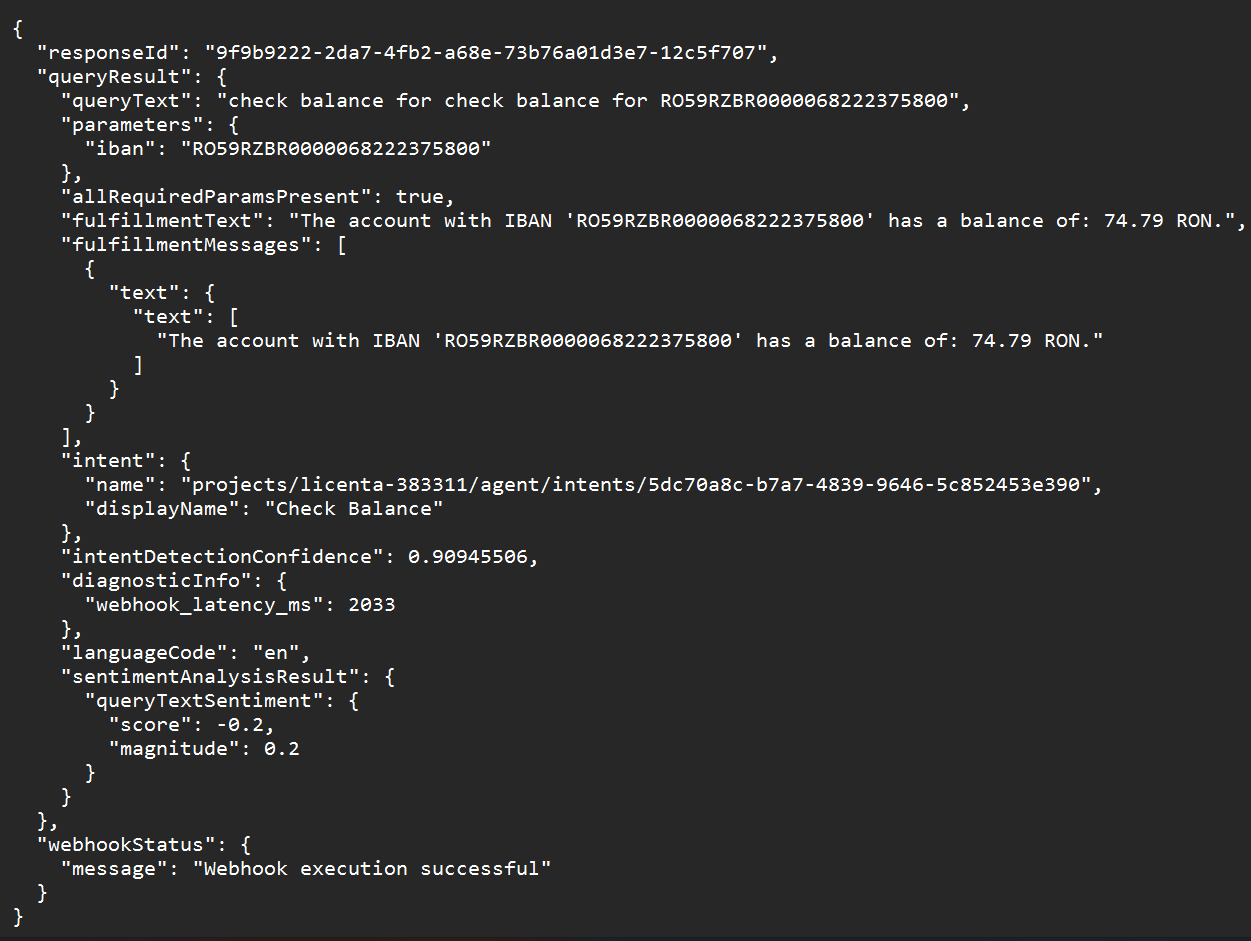
\includegraphics[width=1.0\textwidth]{exemplu-request}
    \caption{Exemplu de request trimis către Google Cloud Function}
    \label{fig:exemplu-request}
\end{figure}

\cleardoublepage

\begin{enumerate}
    \item responseId: acesta este un identificator unic pentru fiecare interacțiune cu DialogFlow.

    \item queryResult: aceasta este secțiunea care conține majoritatea informațiilor legate de interacțiunea cu utilizatorul.
    
    \subitem queryText: aceasta este întrebarea sau afirmația pe care utilizatorul a transmis-o.
    
    \subitem parameters: acestea sunt parametrii extrasi din întrebarea utilizatorului. În acest caz, "iban" este un parametru și valoarea sa este "RO59RZBR0000068222375800".
    
    \subitem allRequiredParamsPresent: acest câmp indică dacă toți parametrii necesari pentru intenție sunt prezenți. În acest caz, este adevărat, ceea ce înseamnă că toți parametrii necesari sunt prezenți.
    
    \subitem fulfillmentText: acesta este textul care va fi returnat utilizatorului ca răspuns la întrebarea sa.
    
    \subitem fulfillmentMessages: aceasta este o listă de mesaje care vor fi trimise înapoi utilizatorului. În acest caz, este doar un mesaj, care este același cu fulfillmentText.
    
    \subitem intent: aceasta este intenția care a fost potrivită pentru întrebarea utilizatorului.
    
    \subitem intentDetectionConfidence: acesta este gradul de încredere cu care DialogFlow a potrivit intenția. În acest caz, este de aproximativ 93%.
    
    \subitem diagnosticInfo: acestea sunt informații suplimentare privind interacțiunea. În acest caz, indică timpul de latență pentru webhook.
    
    \subitem languageCode: acesta este codul de limbă al interogării utilizatorului.
    
    \subitem sentimentAnalysisResult: aceasta este analiza sentimentului textului interogării. Scorul indică sentimentul general (pozitiv sau negativ), iar magnitudinea indică intensitatea sentimentului.
    
    \item webhookStatus: acesta este statusul execuției webhook-ului, care în acest caz a fost reușită.
\end{enumerate}